\documentclass[smallextended]{svjour3}
\usepackage[]{graphicx}\usepackage[]{color}
% maxwidth is the original width if it is less than linewidth
% otherwise use linewidth (to make sure the graphics do not exceed the margin)
\makeatletter
\def\maxwidth{ %
  \ifdim\Gin@nat@width>\linewidth
    \linewidth
  \else
    \Gin@nat@width
  \fi
}
\makeatother

\definecolor{fgcolor}{rgb}{0.345, 0.345, 0.345}
\makeatletter
\@ifundefined{AddToHook}{}{\AddToHook{package/xcolor/after}{\definecolor{fgcolor}{rgb}{0.345, 0.345, 0.345}}}
\makeatother
\newcommand{\hlnum}[1]{\textcolor[rgb]{0.686,0.059,0.569}{#1}}%
\newcommand{\hlstr}[1]{\textcolor[rgb]{0.192,0.494,0.8}{#1}}%
\newcommand{\hlcom}[1]{\textcolor[rgb]{0.678,0.584,0.686}{\textit{#1}}}%
\newcommand{\hlopt}[1]{\textcolor[rgb]{0,0,0}{#1}}%
\newcommand{\hlstd}[1]{\textcolor[rgb]{0.345,0.345,0.345}{#1}}%
\newcommand{\hlkwa}[1]{\textcolor[rgb]{0.161,0.373,0.58}{\textbf{#1}}}%
\newcommand{\hlkwb}[1]{\textcolor[rgb]{0.69,0.353,0.396}{#1}}%
\newcommand{\hlkwc}[1]{\textcolor[rgb]{0.333,0.667,0.333}{#1}}%
\newcommand{\hlkwd}[1]{\textcolor[rgb]{0.737,0.353,0.396}{\textbf{#1}}}%
\let\hlipl\hlkwb

\usepackage{framed}
\makeatletter
\newenvironment{kframe}{%
 \def\at@end@of@kframe{}%
 \ifinner\ifhmode%
  \def\at@end@of@kframe{\end{minipage}}%
  \begin{minipage}{\columnwidth}%
 \fi\fi%
 \def\FrameCommand##1{\hskip\@totalleftmargin \hskip-\fboxsep
 \colorbox{shadecolor}{##1}\hskip-\fboxsep
     % There is no \\@totalrightmargin, so:
     \hskip-\linewidth \hskip-\@totalleftmargin \hskip\columnwidth}%
 \MakeFramed {\advance\hsize-\width
   \@totalleftmargin\z@ \linewidth\hsize
   \@setminipage}}%
 {\par\unskip\endMakeFramed%
 \at@end@of@kframe}
\makeatother

\definecolor{shadecolor}{rgb}{.97, .97, .97}
\definecolor{messagecolor}{rgb}{0, 0, 0}
\definecolor{warningcolor}{rgb}{1, 0, 1}
\definecolor{errorcolor}{rgb}{1, 0, 0}
\makeatletter
\@ifundefined{AddToHook}{}{\AddToHook{package/xcolor/after}{
\definecolor{shadecolor}{rgb}{.97, .97, .97}
\definecolor{messagecolor}{rgb}{0, 0, 0}
\definecolor{warningcolor}{rgb}{1, 0, 1}
\definecolor{errorcolor}{rgb}{1, 0, 0}
}}
\makeatother
\newenvironment{knitrout}{}{} % an empty environment to be redefined in TeX

\usepackage{alltt}
\newcommand{\SweaveOpts}[1]{}  % do not interfere with LaTeX
\newcommand{\SweaveInput}[1]{} % because they are not real TeX commands
\newcommand{\Sexpr}[1]{}       % will only be parsed by R

    
\smartqed  % flush right qed marks, e.g. at end of proof

\usepackage[colorlinks=true,linkcolor={blue},citecolor={blue},urlcolor={blue}]{hyperref}
%\usepackage{caption}
% Add longtable and ctable packages
\usepackage{longtable,ctable}
\usepackage{amsmath}
\usepackage{amssymb}
\usepackage{amsfonts}
\usepackage{multirow}
%\usepackage{amsthm}
\usepackage{graphicx}

\usepackage{booktabs}
%\usepackage{bookmark}

%\usepackage{caption}
%\usepackage{capt-of}

\usepackage{amsmath}
\usepackage{graphicx}
\usepackage{mathptmx}
\usepackage{natbib}

\usepackage{setspace}

%\usepackage{tikz-feynman}
%\usepackage{tikz} 
%\usetikzlibrary{positioning}
\usepackage[utf8]{inputenc}
\usepackage{pgf}


\usepackage{algorithm}
\usepackage{algpseudocode}
\usepackage{enumerate}


\raggedbottom

%\def\convp{\stackrel{p}\rightarrow}
%\def\barn{\bar{N}}
%\def\bary{\bar{Y}}
%\def\baryj{\bar{Y}_{j}(s)}

%\def\barnt{\bar{N}(t)}
%\def\baryjt{\bar{Y}_{j}(t)}
%\def\baryat{\bar{Y}_{0}(t)}
%\def\barybt{\bar{Y}_{1}(t)}
%\def\barnjt{\bar{N}_{j}(t)}
%\def\barnat{\bar{N}_{0}(t)}
%\def\barnbt{\bar{N}_{1}(t)}
%\def\barajt{\bar{A}_{j}(t)}
%\def\baraat{\bar{A}_{0}(t)}
%\def\barabt{\bar{A}_{1}(t)}


% WLR definitions
\def\Grg{\hbox{G}^{\rho,\gamma}}
\newcommand{\fh}[2]{\ensuremath{\hbox{FH}({{#1},{#2}})}}
\newcommand{\Zfh}[2]{\ensuremath{\hbox{Z}^{{#1},{#2}}}}
\def\Zrg{\hbox{Z}^{\rho,\gamma}}
\newcommand{\lam}[2]{\ensuremath{\lambda^{h}(#1|#2)}}
\newcommand{\barF}[2]{\ensuremath{\bar{F}(#1|#2)}}
\newcommand{\barG}[2]{\ensuremath{\bar{G}(#1|#2)}}

\def\hhat{\hat\theta(\hat{H})}
\def\hchat{\hat\theta(\hat{H}^{c})}
\def\hknow{\hat\theta(H)}
\def\hcknow{\hat\theta(H^{c})}
\def\hplim{\theta^{\dagger}(H)}
\def\hcplim{\theta^{\dagger}(H^{c})}


\def\sumin{\sum_{i=1}^n}
\def\nsumin{n^{-1}\sum_{i=1}^n}

\def\ns{n_{0}+n_{1}}
\def\na{n_{0}}
\def\nb{n_{1}}

\newcommand{\indep}{\perp \!\!\! \perp}


\textheight=9.0in \textwidth=6.0in 
\topmargin=0in
\evensidemargin=0in \oddsidemargin=0in




\begin{document}























As a practical illustration we consider a simulated dataset generated as described in Section \ref{sec:sims}.   In this simulated example there are 
$n=700$ subjects, randomized 1:1, where the underlying (marginal) hazard ratio for the harm population $H$ is 
$\hplim =2.5$, and for the complement $H^{c}$, the (marginal) hazard ratio is $\hcplim =0.65$.  The overall (marginal) hazard ratio is $0.71$.  The underlying proportion of subjects in the harm population $H$ is $\approx 13\%$.  Here the actual number of subjects in the $H$ subgroup is $101$ and the number of subjects in the complement equals $599$.  



\begin{figure}[h!]
\begin{center}
\begin{knitrout}
\definecolor{shadecolor}{rgb}{0.969, 0.969, 0.969}\color{fgcolor}
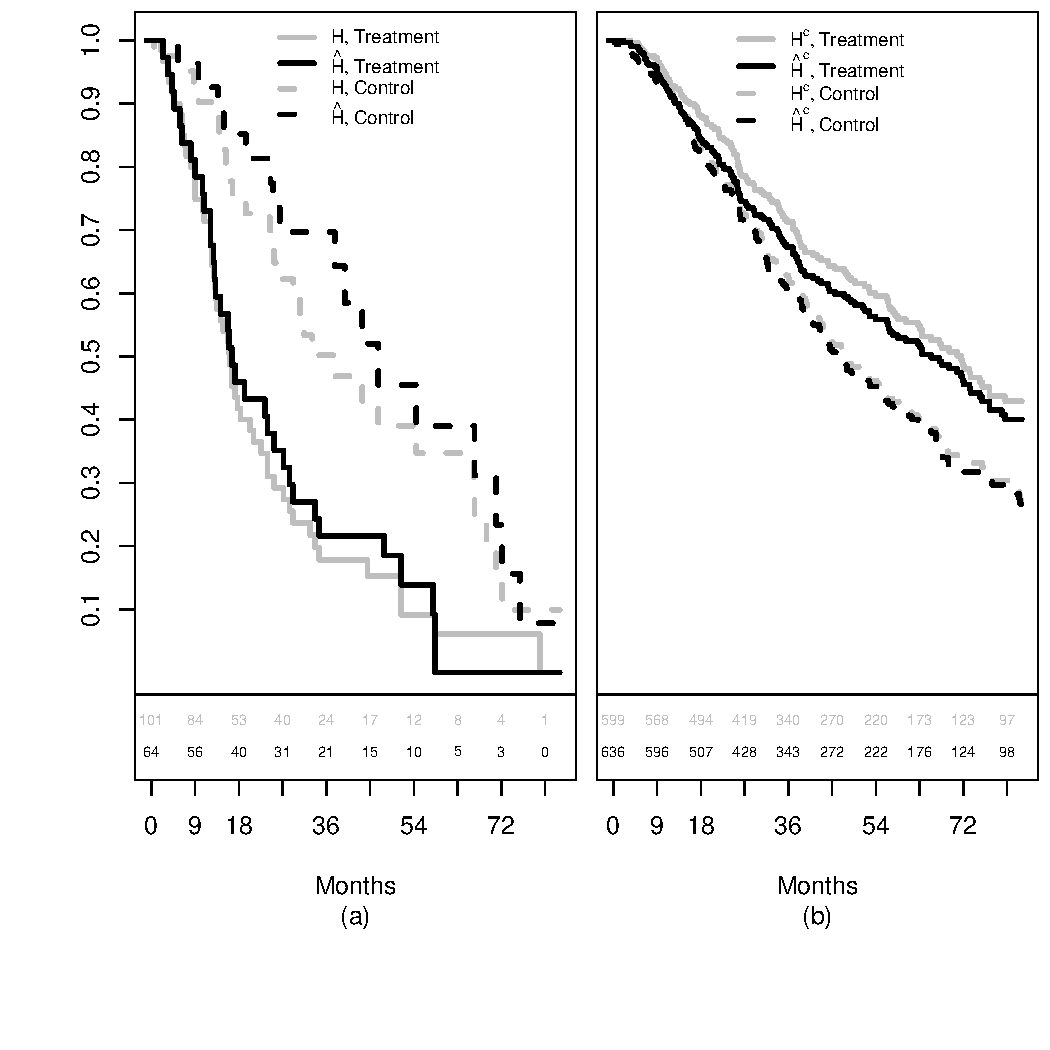
\includegraphics[width=400px,height=200px]{figure/simex1_fig-1} 
\end{knitrout}
\end{center}
\caption{Simulated data example with $\approx 44$\% censoring: (a) Kaplan-Meier (KM) curves for the true $H$ ($H$) subgroup for the treatment (solid grey) 
and control (dashed grey) arms, along with the KM curves for the estimated H ($\hat{H}$) subgroup treatment (solid black) and control (dashed black); 
(b) KM curves for the true complement $H^{c}$ ($H^{c}$) subgroup for the treatment (solid grey) 
and control (dashed grey) arms, along with the KM curves for the estimated $H^{c}$ ($\hat{H}^{c}$) subgroup treatment (solid black) and control (dashed black). The displayed risk sets 
correspond to the treatment and control arms combined for the true and estimated subgroups ($H$ and $\hat{H}$ in (a); $H^{c}$ and $\hat{H}^{c}$ in (b)).}\label{fig:simex1}
\end{figure}



Applying our novel procedure the estimated subgroup $\hat{H}$ consists of $64$ subjects and thus 
$636$ in the estimated complement $\hat{H}^{c}$. The number of subjects in $H$ that are included in $\hat{H}$ is $52$ (i.e., $|H \cap \hat{H}|=52$): Of the $101$ subjects in $H$, $52/101=51\%$ are correctly classified and of the $64$ subjects in $\hat{H}$, $52/64=81\%$ are correctly classified.  For the complement, the number of subjects in $H^{c}$ that are included in $\hat{H}^{c}$ is $587$: Of the $599$ subjects in $H^{c}$, $587/599=98\%$ are correctly classified and of the $636$ subjects in $\hat{H}^{c}$, $587/636=92\%$ are correctly classified.  In the sequel we refer to these as specificity and sensitivity metrics for $\hat{H}$, and $\hat{H}^{c}$.


\begin{table}[!h]

\caption{\label{tab:simex1_tab}\label{tab:simex1} Simulated data example: Cox hazard ratio (hr) estimates for the ITT population and subgroups $H$ and $H^{c}$.
Cox model estimates are based on subgroups: H true (knowing the actual subgroup, a-priori); the estimated subgroup $\hat{H}$; and 
the boostrap bias-correction to $\hat{H}$ estimates, denoted $\hat{H}_{bc}$.  Estimates for the complement $H^{c}$ are defined analogously.
The number of subjects in each population ($\#$ Subjects) and the number of subjects correctly classified in the true subgroups $H$ and $H^{c}$, respectively, are listed ($\#$ Correct).}
\centering
\fontsize{9}{11}\selectfont
\begin{tabular}[t]{lccccc}
\toprule
  & HR Estimate & Lower & Upper & $\#$ Subjects & $\#$ Correct\\
\midrule
\addlinespace[0.3em]
\multicolumn{6}{l}{\textbf{ITT}}\\
\hspace{1em}ITT & 0.838 & 0.687 & 1.021 & 700 & .\\
\addlinespace[0.3em]
\multicolumn{6}{l}{\textbf{H subgroup estimates}}\\
\hspace{1em}H true & 2.358 & 1.471 & 3.781 & 101 & .\\
\hspace{1em}$\hat{H}$ & 3.077 & 1.604 & 5.904 & 64 & 52\\
\hspace{1em}$\hat{H}_{bc}$ & 2.233 & 1.456 & 3.424 & 64 & 52\\
\addlinespace[0.3em]
\multicolumn{6}{l}{\textbf{H-complement subgroup estimates}}\\
\hspace{1em}$H^{c}$ true & 0.672 & 0.537 & 0.841 & 599 & .\\
\hspace{1em}$\hat{H}^{c}$ & 0.733 & 0.592 & 0.908 & 636 & 587\\
\hspace{1em}$\hat{H}^{c}_{bc}$ & 0.744 & 0.593 & 0.933 & 636 & 587\\
\bottomrule
\end{tabular}
\end{table}




Figure \ref{fig:simex1} displays the Kaplan-Meier curves based on the true (known a-priori) subgroups and the estimated subgroups (Figures \ref{fig:simex1}(a) and \ref{fig:simex1}(b), for $H$ and $H^{c}$, respectively).  The Kaplan-Meier curves for the treatment and control arms for the actual subgroups ($H$, known a-prior) are generally well characterized by the estimated subgroups.  


Table \ref{tab:simex1} provides the Cox estimate for the overall population (ITT) as well as the estimates based on the true (known a-priori), and estimated subgroups, $\hat{H}$ and $\hat{H}^{c}$.  The ITT Cox estimate is $0.84$ (95\% CI=$0.69$, $1.02$), 
which is statistically insignificant and highlights the practical implications.  For characterizing $H$, recall that the underlying (marginal) hazard ratio is $\hplim =2.5$.  If the true H is known (a-priori), the Cox estimate is $2.36$ (95\% CI=$1.47$, $3.78$), and for the estimated H, $\hat{H}$, the Cox estimate is $3.08$ (95\% CI=$1.6$, 
$5.9$).  Similar to the model selection area, we expect Cox model estimates based on an estimated subgroup to be optimistic (i.e., upwardly biased for $H$).  We therefore describe a bootstrap bias-correction, which in this case, the bias-corrected Cox estimate denoted by $\hat{H}_{bc}$ is $2.23$ (95\% CI=$1.46$, $3.42$) which we see provides a more ``tempered''estimate and is quite similar to the estimates based on the ideal true H in this simulated example.  
In addition, notice that the CIs for each estimate cover the underlying (marginal) respective hazard ratios 
$\hplim =2.5$ and $\hcplim =0.65$ for $H$ and $H^{c}$, respectively.  
The CIs for $\hat{H}$ and $\hat{H}_{bc}$ also cover the estimate based on $H$ true =  $2.36$; and similarly for the complement where $H^{c}$ true =  $0.67$.  We remark that this simulated example is representative of the results observed in our simulation setting described in Section \ref{sec:sims}.









\bibliographystyle{spbasic}      % basic style, author-year citations
\bibliography{../../subgroups_ref}
\end{document}
